\section{Torsors and principal bundles}

The classical theory of principal bundles tells us to look for an appropriate classifying space of torsors to map into.

\begin{mydef}
Let \( G \) be a group with identity element \( e \) (with the usual classical structure and properties). A \defemph{\( G \)-set} is a set \( X \) equipped with a homomorphism \( \phi:(G,e)\to\Aut(X) \). If in addition we have a term
\[ 
\mathsf{is\_torsor}:||X||_{-1}\times \pit{x:X}\mathsf{is\_equiv}(\phi(-,x):(G,e)\to (X,x))
\] then we call this data a \defemph{\( G \)-torsor}. Denote the type of \( G \)-torsors by \( BG \).
\end{mydef}

If \( (X,\phi),(Y,\psi):BG \) then a \( G \)-equivariant map is a function \( f:X\to Y \) such that \( f(\phi(g,x))=\psi(g,f(x)) \). Denote the type of \( G \)-equivariant maps by \( X\to_G Y \).

\begin{mylemma}
There is a natural equivalence \( (X=_{BG}Y) \simeq (X\to_G Y) \).\qed
\end{mylemma}

Denote by \( * \) the torsor given by \( G \) actions on its underlying set by left-translation. This serves as a basepoint for \( BG \) and we have a group isomorphism \( \Omega BG\simeq G \).

\begin{mylemma}
A \( G \)-set \( (X,\phi) \) is a \( G \)-torsor if and only if there merely exists a \( G \)-equivariant equivalence \( *\to_G X \).\qed
\end{mylemma}

\begin{mycor}
The pointed type \( (BG,*) \) is a \( \K(G,1) \).\qed
\end{mycor}

In particular, to classify principal \( S^1 \)-bundles we map into the space \( \K(S^1, 1) \), a type of torsors of the circle. Since \( S^1 \) is a \( \Kzo \), we have \( \K(S^1,1)\simeq\Kzt \).

\subsection{Bundles of mere circles}

We find it illuminating to look also at the slightly more general classifying space of \( \Kzo \)-bundles, that is bundles whose fiber are equivalent to \( \Kzo \). We can understand very well when these are in fact bundles of circle torsors, which will in turn shed light on orientation in this setting. 

We will follow Scoccola\cite{sco}. We will state the definitions and theorems for a general \( \K(G,n) \) but we will be focusing on \( n=1 \) in this note.

\begin{mydef}
Let \( \EM(G,n)\defeq \BAut(\K(G,n))\defeq \sit{Y:\uni}||Y\simeq \K(G,n)||_{-1}\). A \defemph{\( \K(G,n) \)-bundle} on a type \( M \) is the fiber of a map \( M\to\EM(G,n) \).
\end{mydef}

Scoccola uses two self-maps on the universe: suspension followed by \( (n+1) \)-truncation \( ||\Sigma||_{n+1} \) and forgetting a point \( F_\bullet \) to form the composition 
\[ 
\EM(G,n)\xrightarrow[]{||\Sigma||_{n+1}} \EM_{\bullet\bullet}(G,n+1)\xrightarrow[]{F_\bullet}\EMp(G,n+1)
\]
from types to types with two points (north and south), to pointed types (by forgetting the south point).

\begin{mydef}
Given \( f:M\to\EM(G,n) \), the \defemph{associated action of \( M \) on \( G \)}, denoted by \( f_\bullet \) is defined to be \( f_\bullet=F_\bullet\circ||\Sigma||_{n+1}\circ f \).
\end{mydef}

\begin{mythm}
(Scoccola\cite{sco} Proposition 2.39). A \( \K(G,n) \) bundle \( f:M\to\EM(G,n) \) is equivalent to a map in \( M\to\K(G,n+1) \), and so is a principal fibration, if and only if the associated action \( f_\bullet \) is contractible.
\end{mythm}

Let's relate this to \emph{orientation}. Note that the obstruction in the theorem is about a map into \( \EMp(G,n+1) \) and further note that \( \EMp(G,n)\simeq \K(\Aut G,1) \) (independent of \( n \)). The theorem says that the data of a map into \( \EM(G,n) \) factors into data about a map into \( \K(G,n+1) \) and one into \( \K(\Aut G,1) \). Informally, \( \EM(G,n) \) is a little too large to be a \( K(G,n+1) \), as it includes data about automorphisms of \( G \).

In the special case of \( \EMzo \) the conditions of the theorem are met when \( f_\bullet:M\to\K(\Aut \zz, 1) \) is contractible. \( \Aut\zz \) consists of the \( \zz/2\zz \) worth of outer automorphisms given by multiplication by \( \pm 1 \). If we look at the fiber sequence
\[ 
\K(S^1, 1)\to \BAut S^1\to \K(\Aut \zz, 1)
\] we see the automorphisms of the circle as an extension of the group of automorphisms that are homotopic to the identity (which are the torsorial actions) by the group that sends the loop in \( S^1 \) to its inverse. This is another way to see that a map \( f:M\to \BAut S^1\simeq \EMzo \) factors through \( \K(S^1, 1)\simeq \Kzt \) if and only if the composition to \( \K(\Aut\zz,1) \) is trivial. This amounts to a choice of loop-direction for all the circles, and so deserves the name ``\( f \) is \emph{oriented}.'' In addition the map \( \BAut S^1\to \K(\Aut \zz, 1) \) deserves to be called the first Stiefel-Whitney class of \( f \), and the requirement here is that it vanishes. This point of view is discussed in Schreiber\cite{dcct} (starting with Example 1.2.138) and in Myers\cite{myersgood}.

\begin{mynote}
Bundles of oriented mere circles are principal, but this fact does not hold for bundles of higher-dimensional spheres. Since this note will focus on 2-dimensional oriented manifolds we will be making use of this coincidence.
\end{mynote}

\subsection{Pathovers in circle bundles}
\label{sec:pathovers}
Suppose we have \( T:M\to\EMzo \) and \( P\defeq\sit{x:M}T(x) \). We adopt a convention of naming objects in \( M \) with Latin letters, and the corresponding structures in \( P \) with Greek letters. Recall that if \( p:a=_M b \) then \( T \) acts on \( p \) with what's called the \emph{action on paths}, denoted \( \ap(T)(p):T(a)=T(b) \). This is a path in the codomain, which in this case is a type of types. Type theory also provides a function called \emph{transport}, denoted \( \tr(p):T(a)\to T(b) \) which acts on the fibers of \( P \). \( \tr(p) \) is a function, acting on the terms of the types \( T(a) \) and \( T(b) \), and univalence tells us this is the isomorphism corresponding to \( \ap(T)(p) \).

Type theory also tells us that paths in \( P \) are given by pairs of paths: a path \( p:a=_M b \) in the base, and a pathover \( \pi:\tr(p)(\alpha)=_{T(b)}\beta \) between \( \alpha:T(a) \) and \( \beta:T(b) \) in the fibers. We can't directly compare \( \alpha \) and \( \beta \) since they are of different types, so we apply transport to one of them. We say \( \pi \) lies over \( p \). See Figure~\ref{fig:pathovers}.

\begin{figure}[H]
\centering
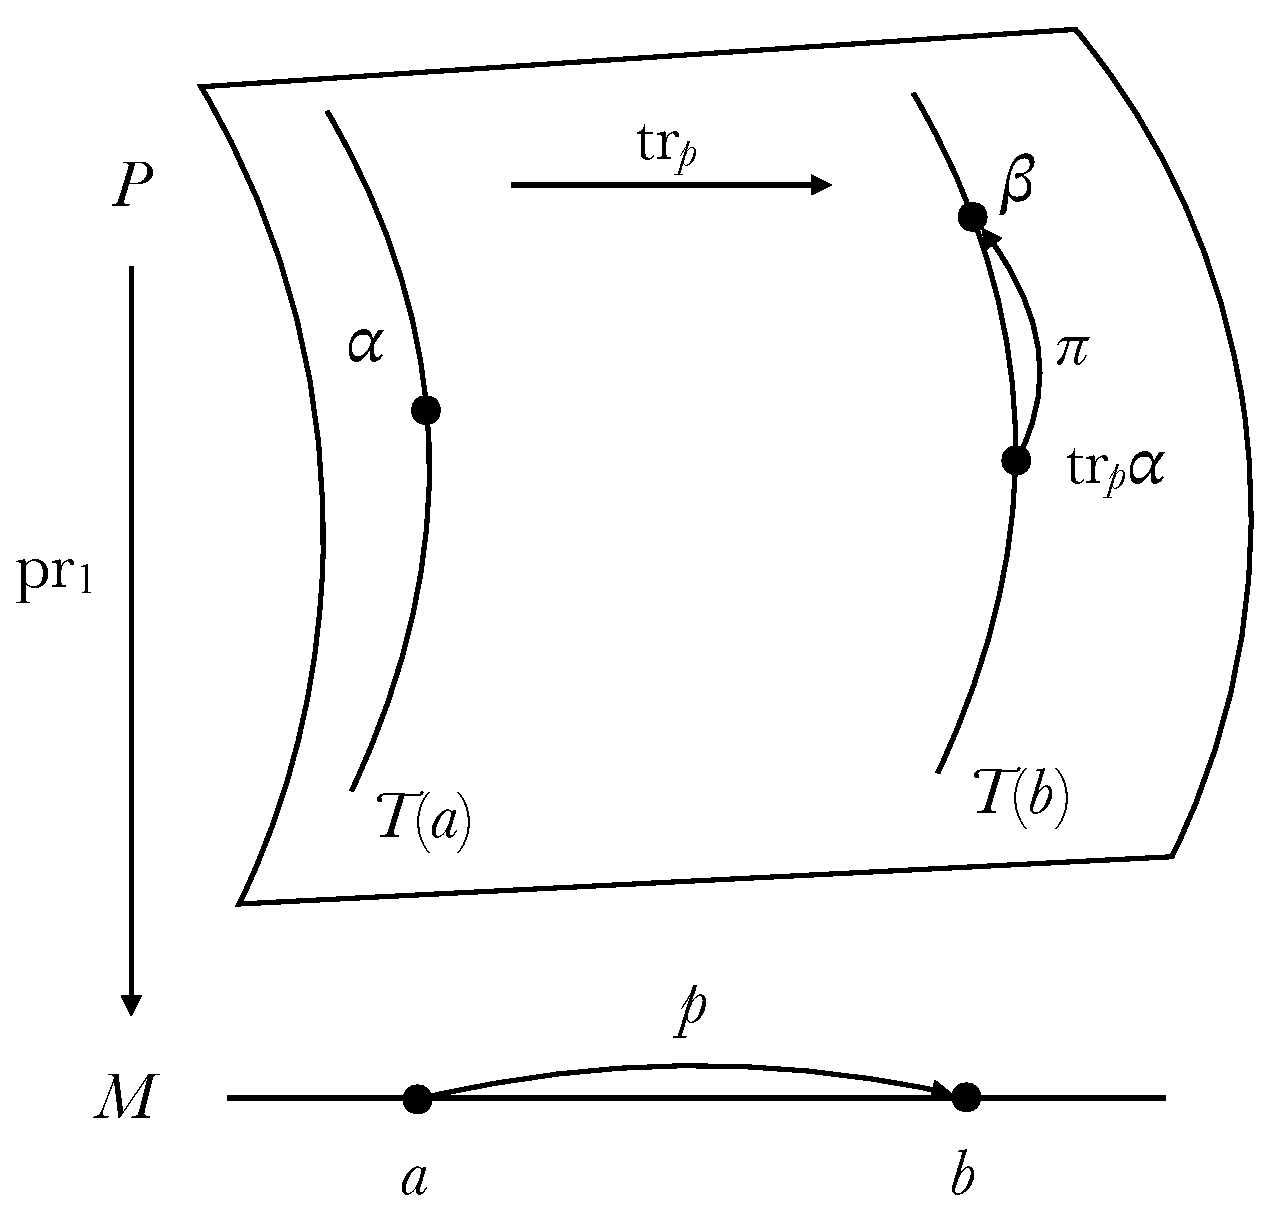
\includegraphics[width=200pt]{figs/pathovers.pdf}
\caption{A path \( \pi \) over the path \( p \) in the base involves the transport function.}
\label{fig:pathovers}
\end{figure}

Lastly we want to recall that in the presence of a section \( X:M\to P \) there is a dependent generalization of \( \ap \) called \( \apd \): \( \apd(X)(p):\tr(p)(X(a))=X(b) \) which is a pathover between the two values of the section over the basepoints of the path \( p \).
